\documentclass{bmstu-gost-7-32}

\begin{document}

\makereporttitle
	{Информатика, искусственный интеллект и системы управления} % Название факультета
	{Программное обеспечение ЭВМ и информационные технологии} % Название кафедры
	{лабораторной работе №~3} % Название работы (в дат. падеже)
	{Конструирование компиляторов} % Название курса (необязательный аргумент)
	{Синтаксический разбор с использованием метода рекурсивного спуска} % Тема работы
	{6} % Номер варианта (необязательный аргумент)
	{ИУ7-23М} % Номер группы
	{Керимов~А.~Ш.} % ФИО студента
	{Ступников~А.~А.} % ФИО преподавателя

\section*{Описание задания}

\textbf{Цель работы:} приобретение практических навыков реализации рекурсивного спуска для синтаксического разбора.

\textbf{Задачи работы:}
\begin{enumerate}
	\item Выбрать грамматику по варианту.
	\item Дополнить грамматику блоком, состоящим из последовательности операторов присваивания.
	\item Для модифицированной грамматики написать программу нисходящего синтаксического анализа с использованием метода рекурсивного спуска.
\end{enumerate}

\textbf{Вариант 1. Грамматика G1}

Рассматривается грамматика выражений отношения с правилами

\begin{verbatim}
	<выражение> ->
	     <простое выражение> |
	     <простое выражение> <операция отношения> <простое выражение>

	<простое выражение> ->
	    <терм> |
	    <знак> <терм> |
	    <простое выражение> <операция типа сложения> <терм>

	<терм> ->
	    <фактор> |
	    <терм> <операция типа умножения> <фактор>

	<фактор> ->
	    <идентификатор> |
	    <константа> |
	    ( < простое выражение > ) |
	    not <фактор>

	<операция отношения> ->
	    = | <> | < | <= | > | >=

	<знак> ->
	    + | -

	<операция типа сложения> ->
	    + | - | or

	<операция типа умножения> ->
	    * | / | div | mod | and
\end{verbatim}

\textbf{Замечания.}

\begin{enumerate}
	\item Нетерминалы <идентификатор> и <константа> — это лексические единицы (лексемы), которые оставлены неопределенными, а при выполнении лабораторной работы можно либо рассматривать их как терминальные символы, либо определить их по своему усмотрению и добавить эти определения.
	\item Терминалы \textbf{not}, \textbf{or}, \textbf{div}, \textbf{mod}, \textbf{and} — ключевые слова (зарезервированные).
	\item Терминалы ( ) — это разделители и символы пунктуации.
	\item Терминалы = <> < <= > >= + - * / — это знаки операций.
	\item Нетерминал <выражение> — это начальный символ грамматики.
\end{enumerate}

\textbf{Вариант в стиле Си}

\begin{verbatim}
	<программа> ->
	    <блок>

	<блок> ->
	    { <список операторов> }
`
	<список операторов>
	    <оператор> <хвост>

	<хвост> ->
	    ; <оператор> <хвост> | eps
\end{verbatim}

Вариант не содержит левую рекурсию, но имеет $\varepsilon$-правило.
Точка с запятой (;) ставится между операторами.
Теперь начальным символом грамматики становится нетерминал <программа>.
Варианта содержит цепное правило <программа> -> <блок>.
Можно начальным символом грамматики назначить нетерминал <блок>. А можно <блок> считать оператором, т. е.

\begin{verbatim}
	<оператор> ->
	    <идентификатор> = <выражение> |
	    <блок>
\end{verbatim}

В последнем случае возможна конструкция с вложенными блоками.
Если между символом присваивания (=) и символом операции отношения (=) возникает конфликт, то можно для любого из них ввести новое изображение, например, :=, <-, == и т. п.

\section*{Текст программы}

С полным текстом программы можно ознакомиться по адресу: \url{https://github.com/wcdbmv/CD/tree/lab03/lab03/src}.

\section*{Тестирование и результаты}

Выражение:
\begin{verbatim}
	{a = -b + const < (not a + b) * b div a; {a = a <> a; {c = const}}}
\end{verbatim}

Результат:

\noindent 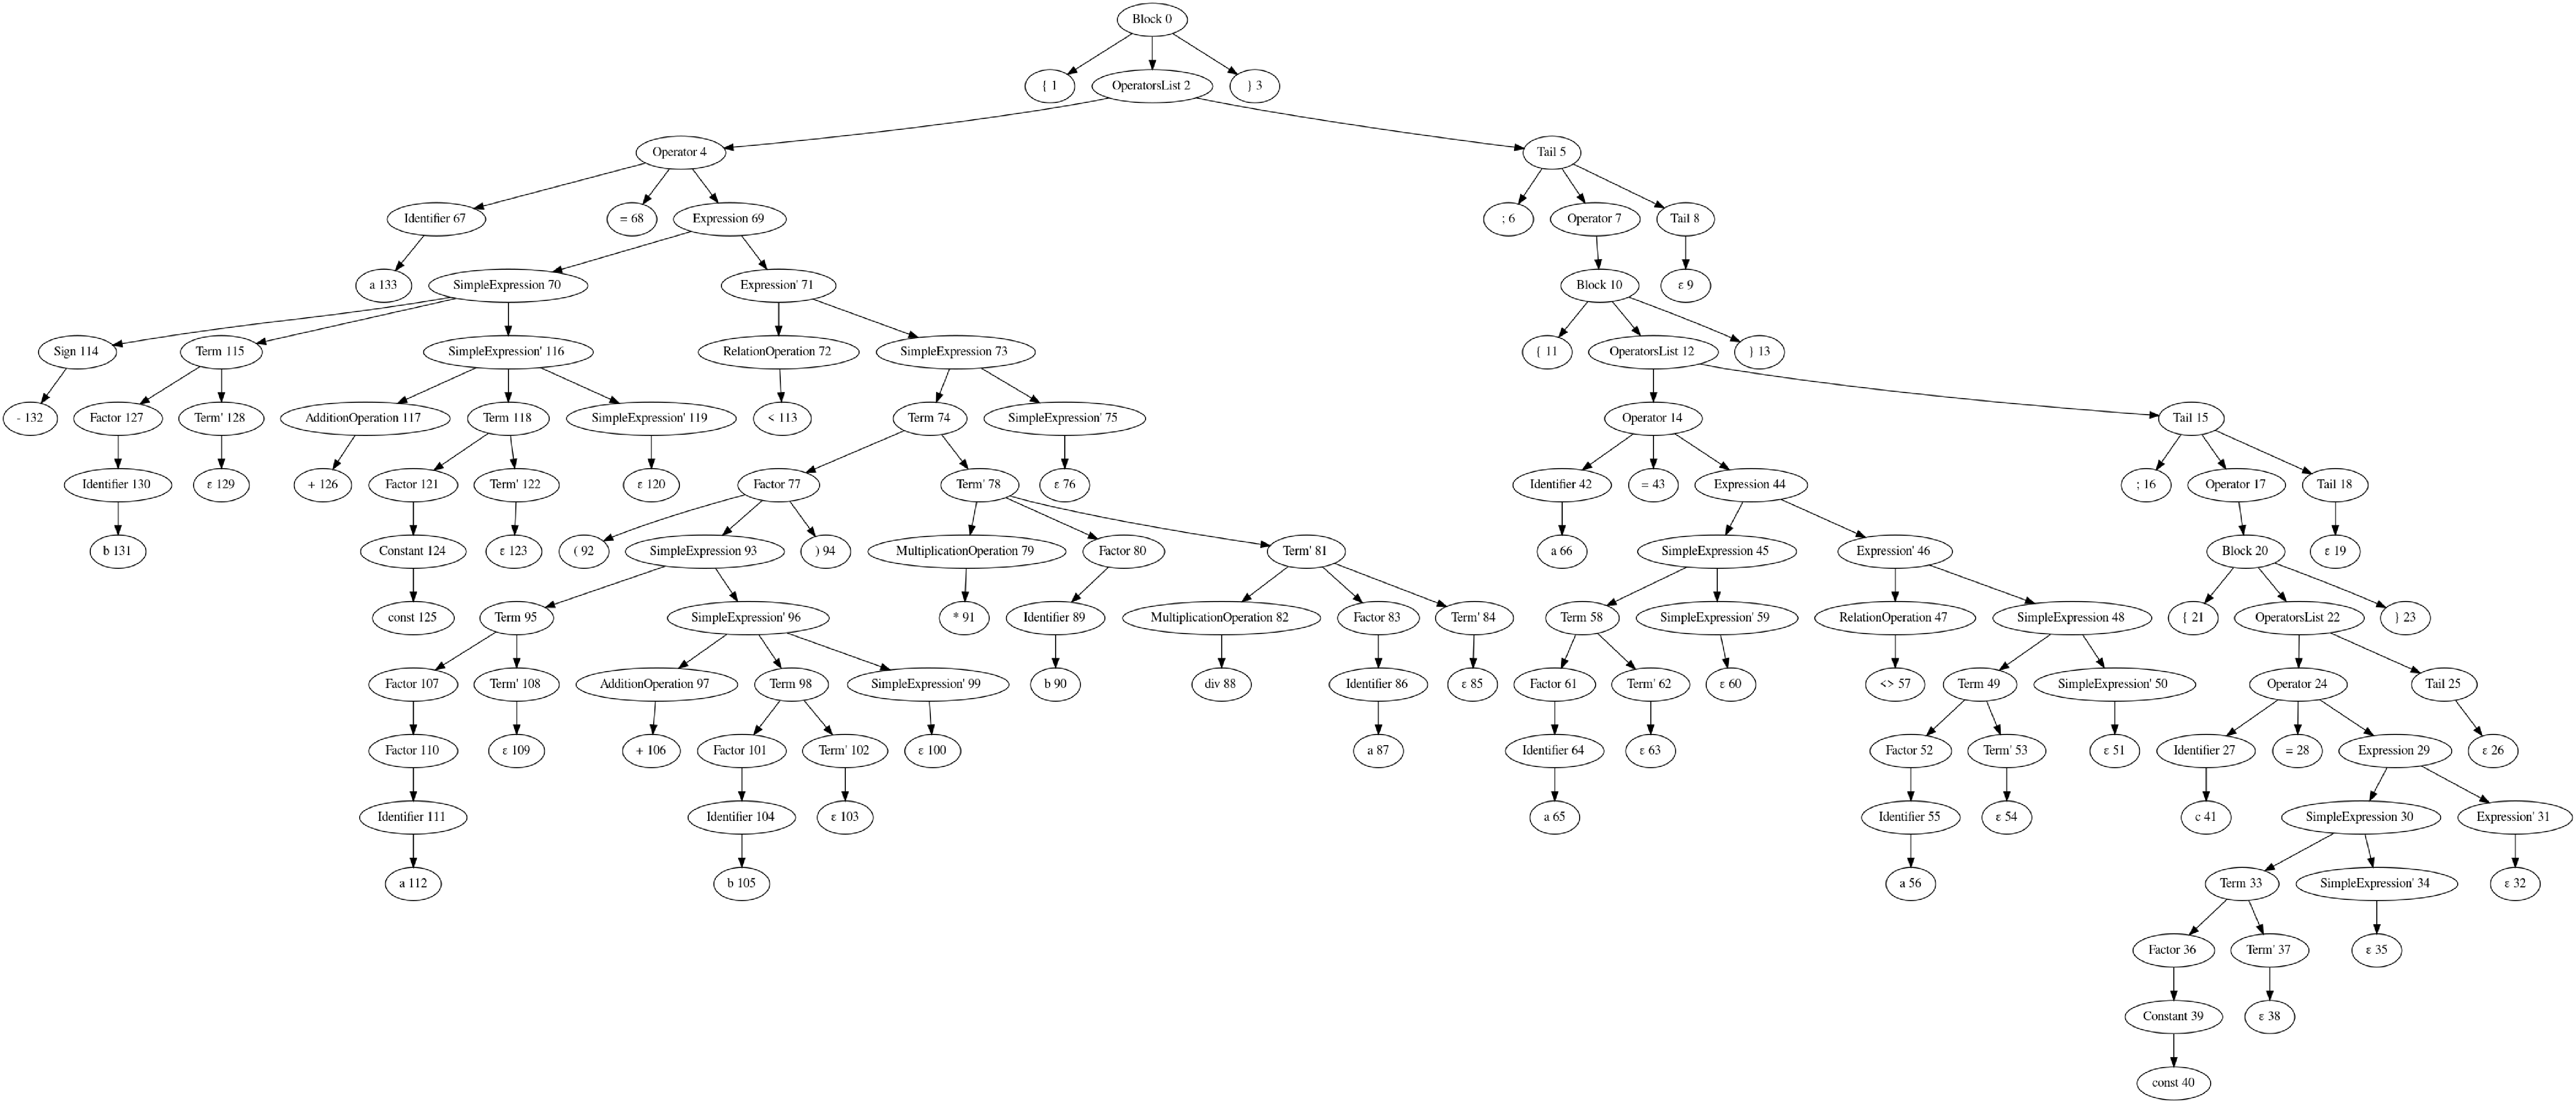
\includegraphics[width=\linewidth]{inc/img/tree}

\section*{Выводы}

В данной работе был реализован метод нисходящего рекурсивного анализа выражения.
Были получены навыки реализации леворекурсивного спуска и проанализированы различные входные данные.

\end{document}
